\cleardoublepage

\lgf{\chapter{Mettre en œuvre un Capteur Virtuel}}
\lge{\chapter{Implementing a Virtual Sensor}}


\lgf{\textit{Les programmes relatifs à cette section se trouvent dans le répertoire \texttt{plido-tp3}. Il est recommandé d'utiliser la machine virtuelle avec une fenêtre de terminal pour l'objet et une autre pour le serveur.}}
\lge{\textit{The programs related to this section are located in the directory \texttt{plido-tp3}. It is recommended to use the virtual machine with one terminal window for the object and another for the server.}}

\section {JSON}

\begin{wrapfigure}{r}{3cm}
\Youtube{https://youtu.be/mRuEiwa7Z74}
\end{wrapfigure}

\lgf{Ca fait longtemps qu'on parle d'Internet des Objets, il est temps de mettre en pratique nos connaissances. On va commencer par une mise en oeuvre simple en Python sur votre machine. Le but dans cette partie est de tester tout ce qu'on a vu sans autre matériel qu'un ordinateur. Nous allons ouvrir deux fenêtres terminal. Dans l'une nous allons faire tourner un programme qui va émuler l'objet avec trois capteurs. Cet objet va communiquer avec un serveur qui va recueillir l'information. La communication se fera en interne avec une socket utilisant l'interface \Index{loopback} (cf. figure~\vref{fig-deux-terminaux}).}
\lge{We've been talking about the Internet of Things for a long time, it's time to put our knowledge into practice. We will start with a simple implementation in Python on your machine. The goal in this part is to test everything we have seen without any other hardware than a computer. We will open two terminal windows. In one we will run a program that will emulate the object with three sensors. This object will communicate with a server that will collect the information. The communication will be done internally with a socket using the interface \Index{loopback} (cf. figure~\vref{fig-deux-terminaux}).}


\begin{figure}[tbp]
\centerline{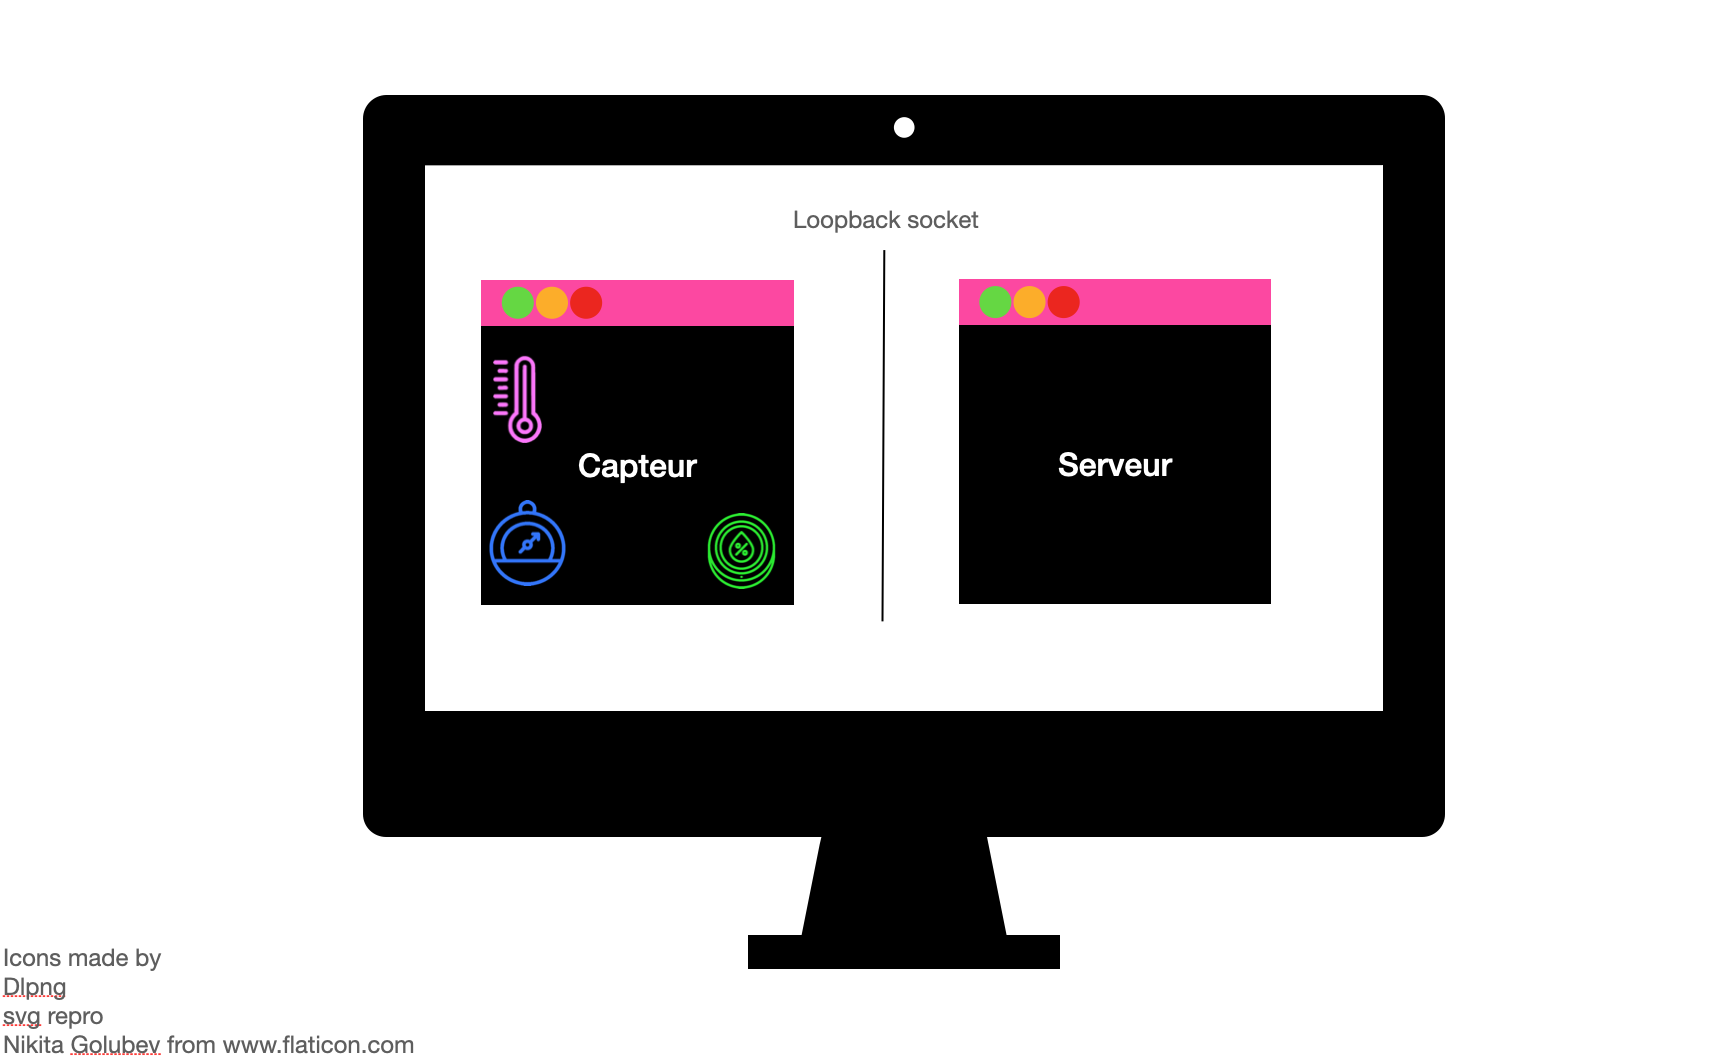
\includegraphics[width=1\columnwidth]{Pictures/Capture24.png}}
\lgf{\caption{Architecture client Serveur}}
\lge{\caption{Client Server architecture}}
\label{fig-deux-terminaux}
\end{figure}

\lgf{\subsection{Serveur Minimal}}
\lge{\subsection{Minimal Server}}
\label{chap-mini-serv}

\pythonlst{minimal\_server.py}


\lgf{Commençons par construire un serveur sommaire (\texttt{minimal\_server.py}) qui va afficher tout ce qu'il reçoit. }
\lge{Let's start by building a summary server (\texttt{minimal\_server.py}) which will display everything it receives. }


\begin{itemize}
    \item 
        \lgf{lignes 1 et 2 les modules \texttt{socket} pour la communication et \texttt{binascii} pour transformer le binaire en chaîne de caractères sont importés.}
        \lge{lines 1 and 2 the modules \texttt{socket} for the communication and \texttt{binascii} to transform the binary into string are imported.}
    \item 
        \lgf{ligne 4, la \pfunction{socket}{socket} crée la socket \texttt{s} avec les paramètres pour des communications IP (\texttt{AF\_INET}) et UDP (\texttt{SOCK\_DGRAM}).}
        \lge{line 4, the socket function creates the socket \texttt{s} with parameters for IP (\texttt{AF\_INET}) and UDP (\texttt{SOCK\_DGRAM}) communications.}
    \item 
        \lgf{ligne 5, la socket est associée au numéro de port \texttt{33033} via la fonction \pfunction{socket}{bind}. L'adresse \texttt{0.0.0.0} indique que les données peuvent venir de n'importe quelle interface (Ethernet, Wi-Fi, loopback,...). }
        \lge{line 5, the socket is associated with the port number \texttt{33033} via the function \pfunction{socket}{bind}. The address \texttt{0.0.0.0} indicates that the data can come from any interface (Ethernet, Wi-Fi, loopback,...). }
    \item 
        \lgf{ligne 8, dans la boucle sans fin, la fonction \pfunction{socket}{recvfrom} va se bloquer dans l'attente de données. Elle retourne les données et l'adresse de l'émetteur.}
        \lge{line 8, in the endless loop, the function \pfunction{socket}{recvfrom} will get stuck waiting for data. It returns the data and the address of the sender.}
    \item 
        \lgf{ligne 9, les données sont affichées en chaîne d'octets et en hexadécimal.}
        \lge{line 9, the data are displayed in byte string and in hexadecimal.}
    
\end{itemize}

     \vspace{1em}

\lgf{On lance le programme serveur. Comme personne lui parle, il n'affiche rien. }
\lge{We launch the server program. As nobody talks to it, it does not display anything. }

\lgf{\subsection{Capteur virtuel}}
\lge{\subsection{Virtual sensor}}

\pythonlst{virtual\_sensor.py}

\lgf{Le module \Index{virtual\_sensor} avec la classe du même nom, reflète de manière à peu près réaliste le comportement d'un capteur. On voit dans le programme principal (ligne 23 à 37) que l'on créé trois capteurs virtuels : un pour la température (ligne 31), un autre pour la pression (ligne 32), et le troisième pour l'humidité (ligne 34). L'argument \texttt{start} précise la valeur de départ, \texttt{variation} la plage de variation entre deux mesures et \texttt{min} et \texttt{max} les valeurs à ne pas dépasser. La boucle sans fin qui affiche les différentes valeurs toutes les secondes.}
\lge{The module \Index{virtual\_sensor} with the class of the same name, reflects in a more or less realistic way the behavior of a sensor. We can see in the main program (line 23 to 37) that we have created three virtual sensors: one for temperature (line 31), another for pressure (line 32), and the third for humidity (line 34). The argument \texttt{start} specifies the starting value, \texttt{variation} the range of variation between two measurements and \texttt{min} and \texttt{max} the values not to exceed. The endless loop that displays the different values every second.}

\begin{termc}[backgroundcolor=\color{palerod}, language=json, basicstyle=\ttfamily\small, escapechar=@]
> @\textbf{python3 virtual\_sensor.py}@
 54.956    999.850  30.609
 54.963   1000.473  32.505
 55.062   1000.845  31.870
 55.017   1001.619  32.257
 55.083   1000.767  31.757
 55.027   1001.442  31.742
 \end{termc} 

\lgf{\subsubsection{Envoi direct}}
\lge{\subsubsection{Direct sending}}


\pythonlst{minimal\_client1.py}

\lgf{Des scripts utilisant ce module peuvent être écrit, comme par exemple le programme \texttt{minimal\_client1.py}.}
\lge{Scripts using this module can be written, as for example the program \texttt{minimal\_client1.py}.}

     \vspace{1em}


\lgf{La variable \texttt{t} contient la température qui est émise sur le port 33033 à l’adresse de \textit{loopback}. On obtient ainsi une communication entre deux programmes dans votre ordinateur dont l'adresse IP locale est \texttt{127.0.0.1}. Mais quand on lance le programme \texttt{minimal\_client1.py}, on obtient l’erreur suivante :}
\lge{The variable \texttt{t} contains the temperature which is transmitted on port 33033 at the \textit{loopback} address. We thus obtain a communication between two programs in your computer whose local IP address is \texttt{127.0.0.1}. But when you launch the program \texttt{minimal\_client1.py}, you get the following error: }


\begin{termc}[backgroundcolor=\color{palerod}, language=json, basicstyle=\ttfamily\small, escapechar=@]
 >python3.5 minimal_client1.py
Traceback (most recent call last):
  File "minimal_client1.py", line 11, in <module>
    s.sendto (t, ("127.0.0.1", 33033))
TypeError: a bytes-like object is required, not 'float'
\end{termc}

\Question{Bug ?}
{
\lgf{Pourquoi le programme client ne fonctionne pas ?}
\lge{Why doesn't the client program work?}

\begin{itemize}[label=$\circ$]
   \item \Wrong{
    \lgf{L’adresse IP n’est pas correcte.}
    \lge{The IP address is not correct.}
    }
   \item \Correct{
    \lgf{Il manque un processus de sérialisation de la donnée.}
    \lge{The data serialization process is missing.}
    }
   \item \Wrong{
    \lgf{La variable \texttt{t} n’est pas définie.}
    \lge{The variable \texttt{t} is not defined.}
    }
   \item \Wrong{
    \lgf{La variable \texttt{t} ne peux pas être lue.}
    \lge{The variable \texttt{t} cannot be read.}
    }
 \end{itemize}
}
{
\lgf{La variable \texttt{t} pointe vers une représentation en mémoire du nombre flottant. Elle ne peut pas être directement envoyée à un autre équipement. Il faut ajouter une phase de sérialisation qui va permettre de transmettre cette information soit en une chaîne de caractères, soit en une chaîne d'octets.}
\lgf{The variable \texttt{t} points to a memory representation of the floating-point number. It cannot be directly sent to another device. It is necessary to add a serialization phase which will make it possible to transmit this information either in a character string, or in a byte string.}
}

\lgf{\subsubsection{Envoi d'une chaîne d'octets}}
\lge{\subsubsection{Sending a byte string}}

\pythonlst[firstline=9,lastline=11, firstnumber=9]{minimal\_client2.py}

\lgf{Dans le programme \texttt{minimal\_client2.py}, le nombre flottant contenu dans la variable \texttt{t} est transformé en chaîne de caractères avec la fonction \texttt{\Index{str}}, puis en chaîne d'octets avec la méthode \pfunction{str}{encode} pour être compatible avec l'argument attendu par la méthode \pfunction{socket}{sendto}. Coté serveur la fonction \texttt{\Index{str}} converti la chaîne d'octets reçue en flottant.}
\lge{In the program \texttt{minimal\_client2.py}, the floating number contained in the variable \texttt{t} is transformed into character string with the function \texttt{Index{str}}, then into bytes string with the method \pfunction{str}{encode} to be compatible with the argument expected by the method \pfunction{socket}{sendto}. On the server side the function \texttt{Index{str}} converts the received byte string into a float.}


\lgf{\subsubsection{Envoi de plusieurs valeurs}}
\lge{\subsubsection{Sending several values}}

\pythonlst[firstline=11,lastline=17, firstnumber=11]{minimal\_client3.py} % 

\lgf{Pour envoyer simultanément les valeurs des trois capteurs, la représentation via une chaîne de caractères est un peu plus compliquée à mettre en oeuvre. Si le programme \texttt{minimal\_client3.py} utilise \pfunction{str}{format} pour envoyer des données séparées par des vigules. Côté serveur, il faut décoder cette chaîne pour y retrouver les entiers. Et ça c'est beaucoup plus complexe à faire ! }
\lge{To send simultaneously the values of the three sensors, the representation via a string is a little more complicated to implement. If the program \texttt{minimal\_client3.py} uses \pfunction{str}{format} to send data separated by vigulas. On the server side, you have to decode this string to find the integers. And this is much more complex to do ! }

\subsubsection{JSON}

\pythonlst[firstline=12,lastline=19, firstnumber=12]{minimal\_client4.py} %

\lgf{La solution la plus simple est de mettre ces trois valeurs dans un tableau python et de le transformer en une représentation JSON grâce à la fonction \pfunction{json}{dumps} du module \texttt{json}. }
\lge{The simplest solution is to put these three values in a python array and transform it into a JSON representation using the \pfunction{json}{dumps} function of the \texttt{json} module. }

     \vspace{1em}

\lgf{Cette chaîne de caractères JSON est à son tour transformée en chaîne d'octets avec encode et envoyée au serveur. Dans notre cas, le serveur ne fait qu'afficher la chaîne de caractères mais vous pouvez utiliser la méthode \pfunction{json}{loads} du module \texttt{json} pour desérialiser et en faire une structure Python dans le serveur, sur laquelle il est maintenant facile d'effectuer des opérations comme, par exemple, un calcul de moyenne.}
\lge{This JSON string is in turn transformed into a byte string with encoding and sent to the server. In our case, the server only displays the string but you can use the \pfunction{json}{loads} method of the \texttt{json} module to deserialize it and turn it into a Python structure in the server, on which it is now easy to perform operations such as, for example, an average calculation.}

\begin{termc}[backgroundcolor=\color{palerod}, language=json, basicstyle=\ttfamily\tiny, escapechar=@]
% @\textbf{python3 minimal\_server.py}@
b'[19.93044784157464, 999.1552628155773, 35.723583473834566]' => b'5b31392e39333034343738343135373436342c203939392e313535c...
b'[19.940155545405723, 998.7581534530281, 35.820037116376184]' => b'5b31392e3934303135353534353430353732332c203939382e3735...
b'[20.003803212269627, 999.3517302791449, 34.33544522779677]' => b'5b32302e3030333830333231323236393632372c203939392e33353...
\end{termc}

\section{CBOR}

\begin{wrapfigure}{r}{3cm}
\Youtube{https://youtu.be/PmudahiRWFw}
\end{wrapfigure}

\lgf{Le passage de JSON à CBOR est très simple. Il suffit de changer un module \texttt{cbor} à la place du module de \texttt{json}. Le programme \texttt{minimal\_client5.py}~:}
\lge{The passage from JSON to CBOR is very simple. It is enough to change a module \texttt{cbor} instead of the module of \texttt{json}. The program \texttt{minimal\_client5.py}:}

\begin{itemize}
    \item 
        \lgf{ligne 1 fait appel au module cbor2 en le renommant cbor}
        \lge{line 1 calls the cbor2 module and renames it cbor}
    \item 
        \lgf{le reste du programme est identique au précédent, ce n'est que dans la la sérialisation, ligne 18, que la fonction \texttt{json.\pfunction{json}{dumps}} est remplacée par \texttt{cbor.\pfunction{cbor2}{dumps}}. Le format retourné étant une chaîne d'octets, il n'est plus nécessaire de faire appel à la méthode \texttt{encode}.}
        \lge{The rest of the program is identical to the previous one, it is only in the serialization, line 18, that the function \texttt{json.\pfunction{json}{dumps}} is replaced by \texttt{cbor.\pfunction{cbor2}{dumps}}. The format returned being a string of bytes, it is no longer necessary to call the \texttt{encode} method.}
\end{itemize}


     \vspace{1em}


\lgf{Le programme \pprog{minimal\_server.py}{plido-tp3} n'est pas modifié puisqu'il ne fait qu'afficher ce qu'il reçoit. }
\lge{The program \pprog{minimal\_server.py}{plido-tp3} is not modified since it only displays what it receives. }







\begin{termc}[backgroundcolor=\color{palerod}, language=json, basicstyle=\ttfamily\small, escapechar=#]
> #\texttbf{python3 minimal\_server.py}#
b'\x83... => b'83fb40341086f3e8b66bfb408f3b7791c8d61ffb403fac15ba06088e'
b'\x83... => b'83fb40341d4d28495268fb408f33d502185c3dfb403d95a2c4981444'
\end{termc}


\pythonlst{minimal\_client5.py}

\lgf{On obtient le résultat suivant. La séquence CBOR fait 28 octets de long, l'équivalant JSON aurait fait 60 octets. Même si cela divise par deux la taille des données à transmettre, le résultat n'est pas compact. Cela tient à la représentation des nombres flottants en CBOR, car ici les flottant sont codés sur 8 octets.}
\lge{We get the following result. The CBOR sequence is 28 bytes long, the JSON equivalent would have been 60 bytes. Even if this divides by two the size of the data to be transmitted, the result is not compact. This is due to the representation of floats in CBOR, because here floats are coded on 8 bytes.}

\Question{\lgf{Décodage}\lge{Decoding}}
{
\lgf{Analysons la séquence reçue~:}
\lge{Let us analyze the received sequence:}
\texttt{83fb40341086f3e8b66bfb408f3b7791c8d61ffb403fac 15ba06088e}

\lgf{À quoi correspond l’octet 0x83 qui commence la structure CBOR reçue ?}
\lge{What does the byte 0x83 that starts the received CBOR structure correspond to?}

\begin{itemize}[label=$\circ$]
   \item \Wrong{
    \lgf{au codage de l'entier positif 131.}
    \lge{to the coding of the positive integer 131.}
    }
   \item \Wrong{
    \lgf{au codage de l'entier négatif 132.}
    \lge{to the coding of the negative integer 132.}
    }
   \item \Correct{
    \lgf{à la définition d'un tableau de 3 éléments.́}
    \lge{to the definition of an array of 3 elements.́}
    }
   \item \Wrong{
    \lgf{à la définition d'un map CBOR de 3 éléments.}
    \lge{the definition of a CBOR map of 3 elements.}
    }
   \item \Wrong{
    \lgf{à la définition d'un tableau de taille non définie.}
    \lge{to the definition of an array of undefined size.}
    }
 \end{itemize}
 }
 {
 \lgf{0x83 s'écrit en binaire \texttt{100-0 0111}. \texttt{100} est le type majeur pour un tableau. La valeur \texttt{00111} est inférieure à 24. Il s'agit donc du nombre d'éléments du tableau, donc un tableau de 3 éléments.}
 \lge{0x83 is written in binary \texttt{100-0 0111}. \texttt{100} is the major type for an array. The value \texttt{00111} is lower than 24. It is thus the number of elements of the array, thus an array of 3 elements.}

 }

\Question{\lgf{Flottant}\lge{Floating}}
{
\lgf{Dans cette structure, quel est le marqueur CBOR (en hexadécimal) qui indique que l’on a un nombre flottant ?}
\lge{In this structure, what is the CBOR marker (in hexadecimal) that indicates that we have a floating number?}
}
{
\lgf{0xFB, si on l'écrit en binaire on obtient \texttt{111-1 1100}. Le majeur correspond à la catégorie des flottant et des valeurs spéciales.}
\lge{0xFB, if we write it in binary we obtain \texttt{111-1 1100}. The major corresponds to the category of floats and special values.}
}

\Question{\lgf{Taille du flottant}\lge{Floating size}}
{
\lgf{Quelle est la taille de ce flottant en octets ?}
\lge{What is the size of this floating number in bytes?}
}
{
\lgf{8 octets~; la partie mineur \texttt{1 1100} indique qu'il s'agit d'un flottant codé sur 8 octets}
\lge{8 bytes; the minor part \texttt{1 1100} indicates that it is a float coded on 8 bytes}
}

\lgf{\subsubsection{Utilisation de nombres entiers}}
\lge{\subsubsection{Use of integers}}

\lgf{Pour réduire la taille des données transmises, nous allons utiliser des nombres entiers. Nous aurons besoin d’une précision au centième (deux chiffres après la virgule). Pour ce faire, il suffit, du coté du client, de prendre la partie entière du nombre multiplié par 100 et, du côté du serveur, de diviser la valeur reçue par 100. La modification du code est mineure.}
\lge{To reduce the size of the transmitted data, we will use integers. We will need a precision to the hundredth (two digits after the decimal point). To do this, on the client side, we just take the integer part of the number multiplied by 100 and on the server side, we divide the received value by 100. The modification of the code is minor.}

\pythonlst[firstline=17,lastline=18, firstnumber=17]{minimal\_client6.py}


\begin{termc}[backgroundcolor=\color{palerod}, language=json, basicstyle=\ttfamily\tiny, escapechar=#]
> #\texttbf{python3 minimal\_server.py}#
b'\x83\x19\x07\xd7\x1a\x00\x01\x86O\x19\x0c\xa7' => b'831907d71a0001864f190ca7'
b'\x83\x19\x07\xd4\x1a\x00\x01\x86f\x19\x0cJ' => b'831907d41a00018666190c4a'
b'\x83\x19\x07\xd4\x1a\x00\x01\x86\x92\x19\rP' => b'831907d41a00018692190d50'
\end{termc}

\lgf{La modification est mineure et tient en 12 octets, mais il y a une diminution au niveau de l'interopérabilité, car les deux entités doivent connaître la transformation de la valeur liée à la multiplication par 100.}
\lge{The change is minor and fits in 12 bytes, but there is a decrease in interoperability, as both entities need to know the transformation of the value related to the multiplication by 100.}


\Question{\lgf{Anticipons la taille}\lgf{Anticipating the size}}
{ 
\lgf{Quelle est la taille minimale et maximale de la structure CBOR envoyée, en prenant en compte les valeurs possibles.}
\lge{What is the minimum and maximum size of the CBOR structure sent, taking into account the possible values.}
}
{
\begin{itemize}
    \item 
        \lgf{La température peut évoluer raisonnablement entre -30 et +50, soit -3000 et +5000 après la transformation en entier. La taille minimale, si on envoie 0, la taille sera d'un octet. La taille maximale tiennent sur 3 octets (1 pour le type/longueur et 2 pour les valeurs) }
        \lge{The temperature can reasonably be between -30 and +50, that is to say -3000 and +5000 after the transformation into an integer. The minimum size, if we send 0, the size will be one byte. The maximum size is 3 bytes (1 for the type/length and 2 for the values) }
    \item 
        \lgf{La pression évolue autour de 1000, soit 100~000 après la transformation en entier. La taille sera toujours de 5 octets (1 pour le type/longueur, 4 pour les valeurs)}
        \lge{The pressure evolves around 1000, that is 100~000 after the transformation to integer. The size will always be 5 bytes (1 for the type/length, 4 for the values)}
    \item 
        \lgf{Le taux d'humidité évolue entre 0 et 100 , soit 0 et 10 000 après la transformation en entier. L a taille entre 1 octet et 3 octets.}
        \lge{The moisture content evolves between 0 and 100 , or 0 and 10 000 after the transformation in integer. The size is between 1 byte and 3 bytes.}
\end{itemize}

\lgf{Si on ajoute le type/longueur 0x83 pour indiquer un tableau de trois éléments, on obtient une taille minimale de 1+1+5+1= 8 octets et une taille maximale de 1+3+5+3 = 12 octets.}
\lge{If we add the type/length 0x83 to indicate an array of three elements, we obtain a minimum size of 1+1+5+1= 8 bytes and a maximum size of 1+3+5+3 = 12 bytes.}

}
